\section{Introduction}
\subsection{Background: reading the measurement after failure}
Set reconciliation requires the two parties to recover the symmetric difference of their sets $A$ and $B$.
Database consistency verification is a canonical scenario: each side scans the whole table, compresses every row into a short fingerprint, and comparing the two tables then reduces to computing the symmetric difference of the two fingerprint sets. The number of differing elements $d=|A\triangle B|$ is unknown in advance,
and can vary by several orders of magnitude at different points in time for the same table. The protocol aims to finish in as few rounds as possible while not transmitting a sketch much larger than necessary.

The Invertible Bloom Lookup Table (IBLT) is a common structure for this task. It has $M$ cells, and each cell
stores a count, a key sum, and a checksum. Each element hashes to $k$ distinct cells and adds itself to those cells. Each side builds a
sketch and then the two sketches are subtracted cell by cell; the elements shared by both sides cancel out, leaving only the differing elements: an element only in $A$ carries sign $+1$, and an element only in $B$
carries sign $-1$. Decoding uses peeling: repeatedly find a cell containing a single differing element, read that element out, and delete it from the $k$ cells
to which it belongs. Viewing cells as vertices and the $k$ cells selected by each element as a hyperedge, peeling deletes edges incident to degree-one vertices on this random $k$-uniform
hypergraph. When the load $d/M$ is below the critical value $\alpha_c$ (approximately $0.818$ for $k=3$\cite{molloy,dw}), peeling deletes every edge with high probability; once the load passes $\alpha_c$,
peeling stalls at a nonempty residual 2-core and decoding fails. The failure probability rises from near zero to near one over an interval of width $M^{-1/2}$
around $\alpha_c$.

The capacity $M$ of the IBLT must be fixed before $d$ is known. Choose it too small and decoding fails, requiring another round; choose it too large and bandwidth and memory are wasted. Reference~\cite{prior}
proposes a self-sizing protocol that proceeds in two rounds. The first round sends a fixed small sketch; when there are few differences peeling succeeds and the round ends,
which is the case in most runs in actual deployments. Peeling failure only means the differing elements cannot be listed one by one; the count array held by the receiver is not lost, and it still records $d$.
Among the $d$ differing elements the numbers carrying $+1$ and $-1$ are written $d_+$ and $d_-$; this composition is called the sign composition, and it is summarized by the
sign imbalance $\rho=(d_+-d_-)/d$: $\rho=\pm1$ means all differences come from one side, and $\rho=0$ means the two sides each contribute half. Write $C_v$ for the count of cell $v$, the sum of the signs of the differing elements in that cell. The count energy
\begin{equation*}
T=\sum_{v}\bigl(C_v-\overline C\bigr)^2,\qquad \overline C=\frac1M\sum_vC_v,
\end{equation*}
can be computed before peeling. Each differing element contributes roughly $k$ to the energy, so $\widehat d=T/[k(1-k/M)]$ is an estimate of $d$;
for any sign composition it is exactly unbiased, with variance $2d(d-1)/(M-1)$. When the first round fails, the protocol reads
$\widehat d$, builds the second-round sketch with a fresh hash, and sets its capacity from $\widehat d$.

The estimate $\widehat d$ has random error, and sizing the capacity directly from $\widehat d$ understates $d$ with probability about one half. The protocol therefore introduces a lower
quantile $q_u<1$ and sets the second-round capacity to $\widehat d/q_u$:
\begin{equation*}
\Pr\bigl[\widehat d\ge q_u d\bigm| F\bigr]\ge1-u,
\end{equation*}
where $F$ is the event that the first-round peeling fails, and deployments take $u=0.01$. A smaller $q_u$ covers more conservatively but wastes space, and a larger one gives insufficient coverage probability,
so $q_u$ must be computed accurately.

Reference~\cite{prior} gives two ways to obtain $q_u$. The first is the chi-square approximation under deep overload:
when $d$ far exceeds the first-round capacity, failure occurs almost surely, conditioning on failure hardly changes the distribution, and the unconditional $\widehat d/d$ with $M$ fixed and
$d\to\infty$ tends to a standardized chi-square $(M-1)$ distribution. The second estimates an empirical
quantile by simulation for each configuration. The former applies only under deep overload; the latter works at any load but must be sampled separately for each configuration and yields no cross-configuration pattern.
What neither answers is the \emph{critical window}\cite{dm}, where failure and success have comparable probability.

\subsection{The problem: selection of the mapping by failure}
The lower quantile $q_u$ of the previous section comes from the unconditional distribution of $\widehat d$, but the protocol uses $\widehat d$ only after the first round has failed. If conditioning on failure changes the distribution of $\widehat d$, then a $q_u$ calibrated from the unconditional distribution no longer gives the correct coverage probability, and the second-round capacity systematically deviates from its target.

Intuitively, the count array is fixed before peeling begins, so the outcome of peeling seems unable to affect $\widehat d$. This intuition misses one point: $\widehat d$ and the success or failure of peeling are both determined by the same random mapping. The protocol reads $\widehat d$ only on mappings that leave a nonempty 2-core, which is equivalent to selecting a subset of all mappings and then measuring. Selection changes the distribution of the mapping, and may change the distribution of $\widehat d$.

Figure~\ref{fig:demo} shows this, and also reveals that the strength of the selection effect depends on the sign composition. Two sign configurations are compared on the same set of mappings (so peeling succeeds or fails identically): under one-sided signs ($\rho=1$) the $\widehat d$ of failing samples shifts right as a whole ($\mathbb E[X\mid F]=+0.609$), while under balanced signs ($\rho=0$) it is nearly unchanged ($\mathbb E[X\mid F]=+0.008$).
\begin{figure}[tbp]
\centering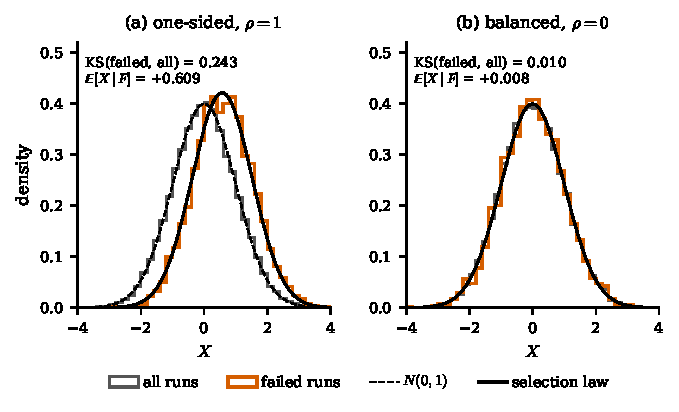
\includegraphics[width=\linewidth]{figures/fig-selection-demo.pdf}
\caption{Selection of the mapping by failure ($k=3$, $M=16384$, failure rate $0.125$, 40,000 Plain hypergraphs). (a) Distribution of $X$ over all samples and over failing samples under one-sided signs, with the solid line the selection law; (b) the same set of hypergraphs with balanced signs.}
\label{fig:demo}
\end{figure}

This dependence has a clear mechanism. The success or failure of peeling depends only on the topology of the hypergraph, not on the signs carried by the elements, but the signs determine how the count energy responds to changes in the topology. When two elements share a cell, equal signs raise the energy and opposite signs lower it. Failure selects hypergraphs with more overlap; when same-sign pairs dominate ($\rho^2$ near one), the extra overlap raises the energy consistently, and the selection effect passes fully to $\widehat d$; when the signs are nearly balanced ($\rho^2$ near zero), the positive and negative contributions cancel, and the selection effect vanishes.

The selection effect is most pronounced inside the critical window. Under deep overload failure is nearly certain, so conditioning on failure hardly selects the mapping; inside the critical window the failure probability rises from zero to one, and the selection is strongest. The magnitude of the bias is controlled by $\rho^2$ and its direction by $k$, so a capacity set from the unconditional $q_u$ may be too large or too small. In database verification the differences produced by replication delay are almost all of one sign, with $\rho^2$ near one, exactly the case of maximal bias.

This paper answers two questions inside the critical window. After the first-round peeling fails, the protocol holds the estimate $\widehat d$ while the true $d$ is unknown. Distribution question: what is the limit distribution of $\widehat d$ conditional on failure, and how does it depend on $k$ and the sign composition. Inference question: how to construct an upper bound on $d$ from the observables available after failure, so that the second-round capacity covers the true difference count with high probability.

\subsection{Main results}

\paragraph{Gaussian-selection law.}
The main result of this paper (Theorem~\ref{thm:main}) gives the limit distribution of the measurement conditional on failure inside the critical window.
We construct a precritical score from the degree profile before peeling begins; it predicts how many degree-one vertices remain when peeling
reaches the bottleneck, and its sign asymptotically determines the success or failure of peeling. Inside the critical window,
the standardized measurement and the precritical score are asymptotically joint Gaussian, with correlation coefficient proportional to $\rho^2$. The measurement conditional on failure is therefore the marginal
of a bivariate normal truncated on a half-plane, which we call the Gaussian-selection law.

The selection effect decays as $\rho^2$: when the signs are asymptotically balanced the conditional distribution returns to the standard normal. The direction of the bias is determined by $k$: for $k=3,4$
the conditional mean is raised, and keeping the unconditional threshold after failure stays on the conservative side; for $k\ge5$
the bias reverses direction, and the same calibration systematically undercovers. The sign change is not obvious: failure always selects hypergraphs with more overlap, but the net contribution of overlap to the count energy changes sign as $k$ crosses a critical value. This sign change means that for different values of $k$ the calibration after failure
must be corrected in opposite directions, and cannot be handled uniformly by a single empirical rule.

\paragraph{Separation of the signs.}
Theorem~\ref{thm:sign} reduces the general sign composition to the all-same-sign case. The measurement decomposes into two asymptotically independent parts: one depends only on the mapping and has magnitude proportional to $\rho^2$; the other comes only from the random assignment of signs on a fixed mapping. Failure selects only the mapping, so it affects only the first part, and the selection effect scales with $\rho^2$.

\paragraph{Upper confidence bound.}
The selection law gives the conditional distribution, but its parameters depend on the unknown $d$ and cannot be used directly to set the capacity. After failure the protocol can observe $b=d_+-d_-$; testing each candidate difference count against the selection law and inverting yields an upper confidence bound on $d$ (Theorem~\ref{thm:upper}). Compared with the two methods described above, this bound is valid inside the critical window, all its parameters are given by analytic constants, it needs no per-configuration simulation, and it does not rely on the deep-overload asymptotic approximation. After adding the mixture law of the two failure mechanisms, the bound covers the whole load axis, and the protocol can calibrate the second-round capacity with a single formula.

\paragraph{Organization.}
Section~\ref{sec:model} fixes the model and the measurement and separates the role of the sign composition from that of the mapping.
Section~\ref{sec:window} establishes the selection law inside the critical window and analyzes how the direction of the bias depends on $k$.
Section~\ref{sec:upper} constructs the upper confidence bound from the selection law, gives the
finite-size implementation rule, and extends it to the whole load axis. Section~\ref{sec:numerics} checks the theoretical predictions one by one and concludes with an end-to-end
test with unknown $d$. Section~\ref{sec:related} discusses related work. Appendix~\ref{app:notation} collects the notation used throughout; Appendices~\ref{sec:main-proof}--\ref{app:loadaxis} give the complete proofs; Appendix~\ref{app:exp} contains supplementary experiments.
